\cleardoublepage
\chapter{PENDAHULUAN}
\label{chap:pendahuluan}

\section{Latar Belakang}

Kawasan perkotaan di negara berkembang saat ini menghadapi tantangan penurunan kualitas udara yang memengaruhi kesehatan masyarakat dan lingkungan. DKI Jakarta, sebagai pusat ekonomi dan administrasi di Indonesia, tercatat memiliki konsentrasi polutan yang fluktuatif dan sering kali melebihi ambang batas aman yang ditetapkan oleh Organisasi Kesehatan Dunia (WHO). Kondisi atmosfer di wilayah beriklim tropis seperti Jakarta dipengaruhi oleh faktor meteorologi serta emisi dari sektor transportasi dan aktivitas konstruksi \autocite{firdaus2023jakarta}. Berdasarkan data historis, tren penurunan kualitas udara ini ditunjukkan oleh kenaikan rata-rata Indeks Kualitas Udara (AQI) sebesar 69\% pada periode observasi tahun 2017 hingga 2020 \autocite{aulia2024air}.

Dari berbagai parameter kualitas udara yang dipantau melalui stasiun pemantauan, partikulat debu halus dengan ukuran diameter aerodinamis kurang dari 10 mikrometer (PM\textsubscript{10}) merupakan polutan yang memerlukan analisis mendalam. Di kawasan perkotaan Jakarta, PM\textsubscript{10} umumnya bersumber dari debu jalan raya, aktivitas konstruksi, dan emisi hasil pembakaran \autocite{carb2025inhalable}. Karakteristik fisik partikulat yang kecil ini berpotensi menembus sistem filtrasi alami saluran pernapasan manusia dan mengendap pada jaringan paru-paru, sehingga memicu risiko gangguan respirasi jangka panjang.

Dampak paparan PM\textsubscript{10} terhadap kesehatan telah didokumentasikan dalam berbagai studi epidemiologi. Penelitian oleh \textcite{zhang2021association} menunjukkan bahwa setiap kenaikan konsentrasi PM\textsubscript{10} sebesar 10 µg/m³ berkaitan dengan kenaikan jumlah kunjungan gawat darurat akibat penyakit kardiovaskular sebesar 0,14\%. Sementara itu, \textcite{kyung2020particulate} menemukan bahwa paparan jangka pendek terhadap PM\textsubscript{10} berkorelasi dengan kenaikan angka rawat inap pasien Penyakit Paru Obstruktif Kronis (PPOK) sebesar 2,7\%. Data rekam medis tersebut menegaskan bahwa penyediaan informasi proyeksi kualitas udara diperlukan untuk mendukung upaya preventif, khususnya bagi kelompok masyarakat rentan.

Sebagai instrumen mitigasi, Pemerintah Indonesia menerapkan Indeks Standar Pencemar Udara (ISPU) untuk menyampaikan status kualitas udara kepada publik, mengacu pada Peraturan Menteri Lingkungan Hidup dan Kehutanan Nomor 14 Tahun 2020 \autocite{permenlhk2020ispu, chaniago2020ispu}. Kendati demikian, mekanisme pelaporan ISPU saat ini bersifat retrospektif, di mana nilai indeks yang dipublikasikan merupakan representasi dari rata-rata konsentrasi polutan selama 24 jam ke belakang \autocite{septiani2024combating}. Akibatnya, informasi yang diterima masyarakat tidak mencerminkan kondisi riil pada waktu penayangan. Guna mengatasi keterbatasan pelaporan yang reaktif tersebut, diperlukan pendekatan prediktif berupa sistem pemodelan yang mampu memproyeksikan konsentrasi polutan untuk satu hari ke depan ($t+1$).

Dalam mengembangkan sistem proyeksi kualitas udara, penerapan algoritma komputasi berbasis \textit{machine learning} banyak diadopsi karena kapasitasnya dalam mengenali pola data lingkungan yang non-linier. Sebagai contoh, \textcite{alarsy2025pm25} menerapkan algoritma \textit{Random Forest} untuk memprediksi polusi di wilayah urban dan menunjukkan karakteristik yang stabil saat memproses data dengan nilai ekstrem (\textit{outliers}). Di samping itu, arsitektur \textit{Deep Learning} seperti \textit{Long Short-Term Memory} (LSTM) juga kerap diteliti untuk pemrosesan data deret waktu jangka panjang \autocite{radjabaycolle2025improving}.

Meski demikian, masing-masing pendekatan memiliki karakteristik batasan tertentu. Model \textit{machine learning} konvensional sering kali mengalami penurunan akurasi saat memetakan tren linier jangka panjang, sementara metode \textit{Deep Learning} memerlukan alokasi sumber daya komputasi dan durasi pelatihan yang relatif besar. Di sisi lain, metode statistik tradisional seperti \textit{Autoregressive Integrated Moving Average} (ARIMA) efektif dalam memodelkan komponen linier dan tren musiman, namun kurang responsif terhadap lonjakan fluktuasi jangka pendek yang drastis \autocite{vasconcelos2025stationarity}. Guna mengompensasi keterbatasan tersebut, integrasi kedua metode ke dalam model hibrida mulai dikembangkan. Studi oleh \textcite{yenkikar2025explainable} menunjukkan bahwa kombinasi \textit{Random Forest} dan ARIMA mampu menghasilkan estimasi kualitas udara dengan koefisien determinasi ($R^2$) mencapai 0,94.

Namun demikian, sebagian besar literatur yang mengimplementasikan model hibrida \textit{Random Forest}-ARIMA \autocite{naz2024two, chen2025hybrid, yunis2024hybridization} umumnya memproses variabel polutan secara langsung tanpa melibatkan tahapan pengayaan informasi fitur (\textit{feature engineering}). Padahal, variabilitas konsentrasi PM\textsubscript{10} secara fisik memiliki ketergantungan pada kondisi temporal sebelumnya (efek \textit{lag}), nilai rata-rata bergerak (\textit{rolling statistics}), serta interaksi kimiawi antar-polutan di atmosfer, seperti interaksi antara karbon monoksida (CO) dan ozon (O\textsubscript{3}). Representasi fitur turunan ini diperlukan agar model dapat menangkap karakteristik dinamika polusi secara lebih komprehensif.

Keterbatasan lain dalam implementasi pemodelan prediktif berbasis \textit{machine learning} adalah karakteristiknya yang menyerupai kotak hitam (\textit{black-box}), sehingga hubungan inferensial internal model sulit diinterpretasikan \autocite{jimenez2024explainable}. Walaupun model hibrida mampu menghasilkan estimasi numerik $PM_{10}$, model tersebut tidak secara langsung mengonfirmasi kontribusi spesifik dari tiap faktor prediktor. Aspek transparansi ini krusial apabila hasil prediksi akan digunakan sebagai basis analisis oleh otoritas terkait. Untuk mengatasi hambatan tersebut, pendekatan \textit{Explainable Artificial Intelligence} (XAI) dapat diintegrasikan. Metode \textit{SHapley Additive exPlanations} (SHAP) merupakan salah satu pendekatan matematis berbasis teori permainan (\textit{game theory}) yang digunakan untuk mengukur dan memvisualisasikan kontribusi marginal masing-masing fitur terhadap hasil keluaran model \autocite{molnar2025shap}.

Untuk mengatasi keterbatasan model tunggal dalam memetakan fluktuasi kualitas udara, penelitian ini menjadikan studi terdahulu yang dilakukan oleh Yenkikar dkk. \autocite{yenkikar2025explainable} sebagai referensi utama dan jangkar metodologis. Yenkikar dkk. berhasil membuktikan keberhasilan arsitektur hibrida sekuensial yang mengombinasikan keunggulan non-parametrik \textit{Random Forest} Regresi dalam menangkap pola non-linier dengan kapasitas model statistik ARIMA dalam mengurai dependensi linier pada deret sisaan galat (\textit{residual}) \autocite{yenkikar2025explainable}. 

Meskipun demikian, terdapat urgensi mendasar mengapa penelitian lanjutan ini perlu dilakukan. Model asli yang dikembangkan oleh Yenkikar dkk. dilatih menggunakan karakteristik atmosfer luar negeri dan parameter lingkungan yang berbeda, serta belum mengasimilasi pengayaan informasi lewat fitur komposit yang mencerminkan interaksi fisikokimia polutan lokal \autocite{yenkikar2025explainable}. Oleh karena itu, batasan utama dari penelitian tugas akhir ini diarahkan pada tahapan analisis dan evaluasi secara mendalam terhadap penerapan arsitektur hibrida tersebut ketika diintegrasikan dengan pilar rekayasa fitur (\textit{feature engineering}) baru untuk konteks wilayah metropolitan tropis DKI Jakarta.

Kebutuhan akan analisis dan evaluasi inilah yang mendasari penentuan judul tugas akhir ini. Proses analisis dilakukan untuk membedah bagaimana 15 fitur komputasional baru—termasuk fitur interaksi gas prekursor dan komponen temporal—memengaruhi sensitivitas pembelahan simpul pohon keputusan. Sementara itu, proses evaluasi difokuskan untuk menguji secara empiris melalui validasi silang temporal apakah koreksi residual ARIMA mampu menekan nilai galat secara signifikan pada lima stasiun pemantau yang memiliki karakteristik heterogenitas spasial. Melalui batasan cakupan analisis dan evaluasi yang transparan ini, keandalan dan efisiensi arsitektur hibrida Yenkikar dkk. dapat diuji validitas dan aplikabilitas riilnya di bawah kondisi fluktuasi polusi udara Jakarta yang volatil \autocite{yenkikar2025explainable}.

\section{Rumusan Masalah}
Berdasarkan latar belakang yang telah diuraikan, rumusan masalah dalam penelitian Tugas Akhir ini difokuskan pada analisis karakteristik pemodelan prediktif untuk memproyeksikan konsentrasi polutan secara harian serta evaluasi performa model hibrida. Permasalahan tersebut dirumuskan ke dalam pertanyaan-pertanyaan berikut:

\begin{enumerate}
   \item Bagaimana merancang model estimasi harian konsentrasi PM\textsubscript{10} di DKI Jakarta untuk memproyeksikan kualitas udara satu hari ke depan ($t+1$)?
   \item Bagaimana mengintegrasikan algoritma \textit{Random Forest} dan ARIMA ke dalam sebuah model hibrida sekuensial untuk memodelkan komponen linier dan non-linier pada data deret waktu?
   \item Bagaimana pengaruh penerapan teknik rekayasa fitur (\textit{feature engineering}), yang meliputi variabel \textit{lag}, statistik berjalan, dan interaksi antarpolutan, terhadap performa galat (\textit{error}) estimasi model hibrida \textit{Random Forest}-ARIMA?
   \item Bagaimana menerapkan metode \textit{SHapley Additive exPlanations} (SHAP) untuk menganalisis dan menggambarkan kontribusi marginal dari masing-masing fitur prediktor terhadap hasil keluaran model hibrida?
\end{enumerate}

\section{Tujuan Penelitian}

Tujuan utama dari penelitian Tugas Akhir ini adalah mengembangkan dan menguji model prediksi harian konsentrasi PM\textsubscript{10} di DKI Jakarta menggunakan pendekatan hibrida \textit{Random Forest}-ARIMA guna mengevaluasi performa galat dan tingkat interpretabilitas model tersebut pada data deret waktu. Secara lebih spesifik, tujuan penelitian ini adalah:
\begin{enumerate}
   \item Mengonstruksi arsitektur model hibrida \textit{Random Forest}-ARIMA dengan menerapkan teknik rekayasa fitur (\textit{feature engineering}) pada dataset kualitas udara Jakarta periode tahun 2010--2025 serta mengevaluasi nilai galat prediksinya.
   \item Menganalisis kontribusi marginal dan pengaruh fitur masukan terhadap hasil estimasi PM\textsubscript{10} menggunakan metode \textit{SHapley Additive exPlanations} (SHAP) untuk memberikan penjelasan internal model yang terstruktur.
\end{enumerate}

\section{Kriteria Keberhasilan}

Untuk mengukur dan mengevaluasi hasil pemodelan ini secara objektif, ditetapkan tiga kriteria evaluasi teknis sebagai berikut:

\begin{enumerate}
   \item {Reduksi Kesalahan Estimasi (Benchmarking):} Model hibrida \textit{Random Forest}-ARIMA yang dikembangkan dapat meminimalkan tingkat kesalahan peramalan. Keberhasilan ini diukur melalui penurunan metrik \textit{Root Mean Square Error} (RMSE) minimal sebesar 15\% jika dibandingkan dengan model \textit{baseline} (ARIMA murni). Batas threshold 15\% ini merujuk pada acuan batas reduksi galat yang representatif dalam evaluasi model deret waktu \autocite{yenkikar2025explainable}.
   \item {Kontribusi Rekayasa Fitur (Studi Ablasi):} Hasil eksperimen studi ablasi menunjukkan secara empiris bahwa pemanfaatan fitur turunan (hasil \textit{feature engineering}) menghasilkan nilai kesalahan prediksi yang lebih rendah jika dibandingkan dengan arsitektur model yang hanya dilatih menggunakan variabel polutan dasar.
   \item {Interpretabilitas Hasil Model (XAI):} Pemodelan dapat diintegrasikan dengan metode SHAP untuk menghasilkan visualisasi kontribusi fitur, baik pada tingkat global maupun lokal. Visualisasi tersebut dapat memetakan arah hubungan dan pengaruh masing-masing fitur masukan terhadap hasil prediksi PM\textsubscript{10} secara logis serta selaras dengan karakteristik fisis kualitas udara.
\end{enumerate}

\section{Manfaat Penelitian}

Penelitian Tugas Akhir ini diharapkan dapat memberikan kontribusi manfaat ilmiah serta aplikatif sebagai berikut:

\begin{enumerate}
   \item Memberikan kajian empiris tambahan mengenai karakteristik pencatatan dan implementasi model hibrida \textit{Random Forest}-ARIMA yang dikombinasikan dengan teknik rekayasa fitur pada data kualitas udara di wilayah urban beriklim tropis.
   \item Menjadi materi referensi ilmiah mengenai pengaruh penggunaan dimensi fitur temporal (\textit{lag} dan \textit{rolling window}) terhadap fluktuasi nilai galat pemodelan deret waktu untuk polutan udara secara berskala.
   \item Menyediakan contoh dokumentasi metodologis terkait penerapan pendekatan \textit{Explainable AI} (XAI) menggunakan analisis SHAP untuk memetakan hubungan kausalitas antarpolutan udara secara terstruktur.
   \item Menghasilkan rancangan konfigurasi model prediksi harian PM\textsubscript{10} yang dapat dijadikan bahan pertimbangan atau komponen awal dalam pengembangan sistem kajian kualitas udara di kawasan perkotaan Jakarta.
   \item Menyediakan data dan analisis kontribusi polutan yang dapat dimanfaatkan oleh analis lingkungan sebagai referensi tambahan dalam memahami faktor-faktor dominan yang memengaruhi dinamika kualitas udara lokal.
   \item Membantu praktisi pemodelan dalam menginterpretasikan perilaku keputusan internal model \textit{machine learning} melalui visualisasi kontribusi fitur yang lebih transparan dan akuntabel.
\end{enumerate}

\section{Kontribusi Penelitian}

Penelitian Tugas Akhir ini memberikan kontribusi teknis dan empiris yang difokuskan pada tiga aspek pengembangan sistem estimasi kualitas udara berikut:

\begin{enumerate}
   \item {Penyusunan Atribut Rekayasa Fitur Temporal dan Komposit:} Penelitian ini berkontribusi dalam menyusun matriks 15 fitur komposit turunan yang menggabungkan dependensi temporal (\textit{lag} dan \textit{rolling statistics}) serta variabel hasil perkalian antarpolutan ($CO \times O_3$). Pendekatan harian ini digunakan untuk menyertakan karakteristik hubungan antarvariabel polutan secara statistik, sebagai alternatif dari pemrosesan variabel dasar secara terpisah.
   \item {Penerapan Konstruksi Model Hibrida Sekuensial:} Penelitian ini berkontribusi pada implementasi model estimasi harian $PM_{10}$ melalui penggabungan algoritma \textit{Random Forest} dan ARIMA secara sekuensial. Metode ini mengeksplorasi pembagian tugas pemrosesan data, di mana algoritma pohon keputusan digunakan untuk memetakan fluktuasi non-linier dari data masukan, sedangkan model statistik ARIMA digunakan untuk mengolah data sisaan (\textit{residual}) guna menguji pengurangan nilai galat peramalan.
   \item {Analisis Transparansi Perilaku Model Menggunakan SHAP:} Penelitian ini berkontribusi dalam pemanfaatan pendekatan \textit{Explainable AI} (XAI) melalui metode \textit{TreeSHAP} untuk menganalisis keputusan internal model hibrida yang bersifat tertutup (\textit{black-box}). Tahapan ini menghasilkan gambaran kuantitatif mengenai bobot kontribusi masing-masing fitur rekayasa terhadap nilai estimasi, sehingga memberikan informasi tambahan yang dapat ditelaah secara logis dalam konteks kualitas udara Jakarta.
\end{enumerate}

\section{Batasan Masalah}

Guna menjaga fokus penelitian serta kejelasan parameter yang dievaluasi, ruang lingkup kajian dalam Tugas Akhir ini dibatasi pada hal-hal berikut:

\newpage

\begin{enumerate}
   \item {Lokasi Geografis dan Stasiun Pemantauan:} Penelitian hanya menggunakan data kualitas udara di wilayah administratif Provinsi DKI Jakarta yang terekam dari lima stasiun pemantauan resmi di bawah pengelolaan otoritas terkait.
   \item {Dataset dan Rentang Waktu:} Data yang digunakan merupakan data sekunder Indeks Standar Pencemar Udara (ISPU) dengan resolusi harian, terhitung mulai tanggal 1 Januari 2010 hingga 28 Februari 2025.
   \item {Variabel Penelitian:} Fitur masukan (prediktor) yang dimasukkan ke dalam model dibatasi pada lima parameter polutan ISPU, yaitu PM\textsubscript{10}, SO\textsubscript{2}, CO, O\textsubscript{3}, dan NO\textsubscript{2}. Parameter PM\textsubscript{10} bertindak sebagai target proyeksi sekaligus sebagai fitur riwayat temporal (\textit{lag feature}). Penelitian ini tidak melibatkan variabel eksternal seperti data meteorologi (curah hujan, kecepatan angin) maupun volume lalu lintas kendaraan.
   \item {Resolusi Prediksi:} Target luaran (\textit{output}) dari model difokuskan pada estimasi tingkat polusi harian untuk satu hari ke depan (\textit{next-day forecast, t+1}), dan tidak mencakup proyeksi berskala per jam (\textit{hourly}) atau waktu nyata (\textit{real-time}).
   \item {Ruang Lingkup Implementasi:} Penelitian ini dibatasi pada siklus evaluasi model secara \textit{offline} (\textit{offline model evaluation}), yang mencakup tahap prapemrosesan data, perancangan konfigurasi model, penyetelan \textit{hyperparameter}, pengamatan metrik evaluasi galat, hingga visualisasi SHAP. Penelitian ini tidak mencakup tahap rekayasa perangkat lunak lanjutan seperti pembuatan antarmuka aplikasi (\textit{dashboard}) maupun implementasi sistem di lingkungan produksi nyata (\textit{deployment}).
\end{enumerate}

\section{Metodologi Penelitian}

Penelitian Tugas Akhir ini menggunakan kerangka kerja \textit{Design Science Research Methodology} (DSRM). DSRM merupakan salah satu kerangka metodologi yang digunakan untuk penelitian di bidang sistem informasi dan sains data yang berfokus pada analisis rancangan objek kajian. Pemilihan metodologi ini didasarkan pada tujuan penelitian untuk mengonstruksi, menguji konfigurasi artefak komputasi, mendemonstrasikan, serta mengevaluasi kinerjanya secara terukur melalui serangkaian eksperimen numerik \autocite{haryanti2022dsrm}. Alur kerangka kerja DSRM tersebut dapat dilihat pada Gambar \ref{gambar:dsrm}.

\newpage

Artefak yang dikembangkan dalam penelitian ini berupa konfigurasi pemodelan hibrida \textit{Random Forest}-ARIMA yang disusun berdasarkan prinsip pemisahan komponen data \autocite{yenkikar2025explainable}. Eksplorasi model ini mencakup tiga karakteristik penyesuaian: Pemanfaatan dataset kualitas udara Jakarta dengan rentang waktu 15 tahun (2010--2025) untuk mengamati konsistensi perilaku model pada variasi tren yang panjang, pengayaan dimensi masukan melalui rekayasa fitur menjadi matriks 15 fitur turunan, dan penempatan parameter PM\textsubscript{10} sebagai target proyeksi keluaran sekaligus sebagai variabel riwayat (\textit{lag}) masukan.

\begin{figure}[h]
 \centering
 \captionsetup{justification=centering}
 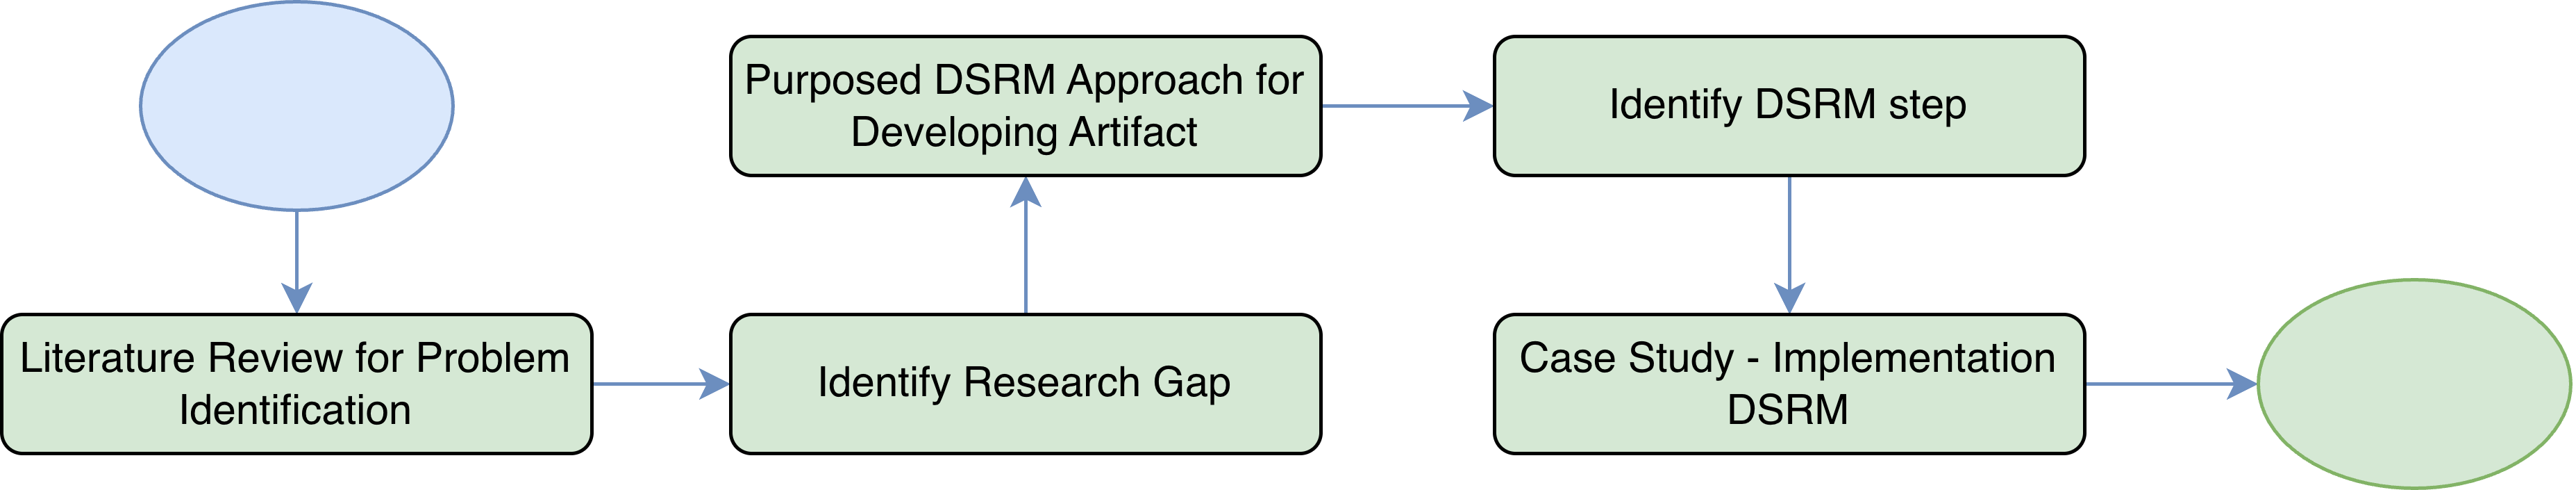
\includegraphics[width=0.8\textwidth]{images/gambar1.png}
 \caption{Kerangka Kerja \textit{Design Science Research Methodology} (DSRM) \autocite{haryanti2022dsrm}}
 \label{gambar:dsrm}
\end{figure}

Guna menjaga keteraturan tahapan penelitian, pelaksanaan DSRM dibagi ke dalam lima langkah sistematis sebagai berikut:

\begin{enumerate}

\item {\textit{Literature Review for Problem Identification}}\\
Tahap awal penelitian meliputi tinjauan pustaka secara sistematis mengenai pemodelan estimasi kualitas udara. Pencarian literatur dilakukan melalui basis data akademik (\textit{Google Scholar, IEEE Xplore, PubMed}) dengan fokus pada publikasi artikel ilmiah terkait periode tahun 2019--2025. Hasil dari tahap ini adalah penetapan karakteristik dasar pemodelan \textit{Random Forest}-ARIMA dari \textcite{yenkikar2025explainable} sebagai referensi struktur hibrida awal yang akan dievaluasi.

\item {\textit{Identify Research Gap}}\\
Tahap ini bertujuan untuk menganalisis karakteristik batasan pada metode eksperimen dari penelitian-penelitian terdahulu. Analisis menunjukkan bahwa sebagian besar pemodelan estimasi masih memproses variabel polutan secara langsung dan belum melibatkan rekayasa fitur temporal yang merepresentasikan akumulasi zat di atmosfer. Kondisi tersebut menjadi landasan untuk menerapkan metode rekayasa fitur komposit pada penelitian ini.

\item {\textit{Proposed DSRM Approach for Developing Artifact}}\\
Tahap ini merupakan proses perancangan konfigurasi komputasi. Arsitektur pemodelan dirancang secara sekuensial: algoritma \textit{Random Forest} digunakan untuk memproses matriks hasil rekayasa fitur guna memetakan pola non-linier, sedangkan fungsi \textit{autoregressive} pada ARIMA bertugas memodelkan komponen linier pada data deret waktu. Tahap ini juga mencakup integrasi pendekatan \textit{SHAP Explainer} agar karakteristik keputusan internal model dapat ditelaah.

\item {\textit{Identify DSRM Step (Execution Procedure)}}\\
Tahap ini merupakan pelaksanaan teknis pemrograman yang mencakup prosedur berikut:
   \begin{enumerate}
       \item \textit{Data Preprocessing}: Rangkaian pembersihan data deret waktu, termasuk penyelarasan data antarstasiun, pengisian nilai kosong (\textit{imputation}), serta penyesuaian rentang nilai (\textit{scaling}).
       \item \textit{Time-Series Feature Engineering}: Ekstraksi fitur masukan menggunakan bahasa pemrograman Python untuk menghasilkan 15 turunan fitur temporal, seperti jeda waktu (\textit{lag}) dan statistik berjalan (\textit{rolling window}).
       \item \textit{Skema Pelatihan Kronologis}: Validasi model menggunakan metode \textit{Time-Series Cross-Validation} (\textit{Forward Chaining}) dengan pembagian rasio data latih dan uji sebesar 80:20 secara berurutan tanpa pengacakan (\textit{shuffle=False}) untuk menghindari risiko kebocoran data masa depan (\textit{look-ahead bias}).
       \item \textit{Hyperparameter Tuning}: Pencarian konfigurasi nilai hiperparameter (seperti parameter jumlah pohon keputusan dan kedalaman maksimum) menggunakan kerangka eksperimen Bayesian pada pustaka Optuna untuk meminimalkan nilai galat.
   \end{enumerate}

\item {\textit{Case Study and Implementation DSRM}}\\
Tahap terakhir adalah implementasi konfigurasi model menggunakan dataset historis ISPU DKI Jakarta \autocite{pohan2025jakarta}. Tahap ini ditujukan untuk mengukur perbandingan performa galat model usulan terhadap model \textit{baseline} (ARIMA murni). Evaluasi diukur melalui persentase penurunan nilai \textit{Root Mean Square Error} (RMSE), serta perbandingan metrik \textit{Mean Absolute Error} (MAE) dan koefisien determinasi ($R^2$). Sebagai analisis akhir, hasil estimasi ditelaah menggunakan grafik \textit{SHAP beeswarm} dan \textit{SHAP dependence}.

\end{enumerate}

\section{Sistematika Penulisan}

Laporan Tugas Akhir ini disusun ke dalam tujuh bab dengan sistematika penulisan sebagai berikut:

\begin{enumerate}
   \item {Bab I Pendahuluan:} Menguraikan latar belakang penurunan kualitas udara, rumusan masalah, tujuan penelitian, kriteria keberhasilan, manfaat penelitian, kontribusi penelitian, batasan masalah, metodologi penelitian, serta sistematika penulisan laporan.
   
   \newpage

   \item {Bab II Studi Literatur:} Menjelaskan pemetaan riset terkait (\textit{state-of-the-art}) dan landasan teori yang mendasari penelitian, meliputi regulasi ISPU, algoritma \textit{Random Forest}, pemodelan deret waktu ARIMA, metode rekayasa fitur, mekanisme kerja Optuna, serta kerangka interpretasi model menggunakan SHAP.
   \item {Bab III Analisis Masalah:} Menyajikan evaluasi terhadap mekanisme pelaporan data yang berjalan, analisis karakteristik dataset kualitas udara Jakarta, analisis pola hubungan empiris polutan, formulasi desain fitur, hingga justifikasi pemilihan solusi prediktif menggunakan \textit{Analytical Hierarchy Process} (AHP).
   \item {Bab IV Perancangan:} Mendeskripsikan arsitektur konseptual pemodelan usulan, desain \textit{data pipeline} eksperimen, spesifikasi algoritmik rekayasa fitur, desain struktur hibrida sekuensial, serta skenario pengujian studi ablasi dan validasi silang.
   \item {Bab V Implementasi:} Mendokumentasikan langkah teknis komputasi pada lingkungan eksperimen yang mencakup eksplorasi data awal, analisis stasioneritas, penerapan rekayasa fitur komposit, pemisahan data latih-uji secara kronologis, hingga kalkulasi fase primer dan sekunder pada model hibrida.
   \item {Bab VI Evaluasi:} Menyajikan metrik evaluasi ekspektasi statistik, pelaporan hasil pengujian studi ablasi, komparasi performa nilai galat antar-model, analisis waktu komputasi pelatihan dan inferensi, serta pembahasan mengenai interpretasi kontribusi fitur menggunakan visualisasi deskriptif SHAP.
   \item {Bab VII Penutup:} Menyampaikan kesimpulan akhir yang ditarik dari hasil evaluasi untuk menjawab pertanyaan penelitian, serta menyajikan saran mengenai keterbatasan dan peluang studi komparatif di masa mendatang.
\end{enumerate}